\documentclass[12pt]{article}
\usepackage{times}
\usepackage{graphicx}
\usepackage{hyperref}
\usepackage{amsmath}
\usepackage{listings}
\usepackage{xcolor}
\usepackage{float}
\usepackage{caption}

\hypersetup{
    colorlinks=true,
    linkcolor=blue,
    urlcolor=blue,
    citecolor=blue,
}

\title{LLM Network Intrusion Detection System}
\author{
    INSyT (Innovative Network Security Technologies)\\
    Taeyang Kim, Bronze Frazer, Isaac Peterson, Damon Tingey\\
    \and
    Sandia National Laboratories\\
    Ryan Holt, Mike Reed\\
}

\date{}

\begin{document}

\maketitle

\begin{abstract}
Current network intrusion detection systems (NIDS) struggle to keep pace with the sophistication and evolving nature of cyberattacks. Traditional signature-based and rule-based systems are often brittle and easily bypassed, while anomaly-based systems suffer from high false positives. This leaves an alarming gap in network security, exposing organizations to data breaches, financial losses, and reputational damage.

We propose the development of a full-stack Large Language Model (LLM) product designed to revolutionize threat analysis through the comprehensive examination of system and network logs as natural language. This solution aims to provide systems that can understand complex attack protocols, detect novel attacks, and adapt to evolving threats. Our system enhances security with proactive and comprehensive defense against a wider range of threats, improves efficiency through accurate threat detection and reduced false positives, and offers a future-proofed defense with continuous adaptation to evolving threats, ensuring long-term effectiveness and protection against emerging attack vectors.
\end{abstract}

\section{Introduction}

Network intrusion is a critical issue in today's digital landscape. In 2023, the average cost per data breach in the United States was \$9,480,000 \cite{databreachreport}. Organizations face significant financial losses, operational disruptions, and reputational damage due to sophisticated cyberattacks that traditional NIDS struggle to detect effectively.

Current NIDS rely heavily on signature-based and rule-based methodologies, which are often inflexible and unable to detect novel or sophisticated attacks \cite{traditionalnids}. Anomaly-based systems, while more adaptive, tend to generate high false-positive rates, burdening security teams with excessive alerts \cite{anomalyissues}.

To address these challenges, we propose a novel approach: leveraging advanced LLMs to analyze system and network logs as natural language, enabling a deeper understanding of complex attack patterns and the detection of previously unseen threats.

\section{Related Work}

Machine learning has been applied to NIDS with varying degrees of success. Previous work has explored the use of neural networks for intrusion detection \cite{neuralnids}, but they often lack the ability to interpret the semantic content of log data effectively. Recent advancements in Natural Language Processing (NLP) and LLMs, such as BERT \cite{bert}, have shown promise in interpreting and classifying text data, which can be applied to system logs.

Our approach distinguishes itself by treating log data as a form of pseudo-natural language, allowing the LLM to learn patterns and correlations that traditional models may miss.

\section{Methodology}

\subsection{System Overview}

Our proposed system is a full-stack framework capable of classifying network intrusions using LLMs. The key components include:

\begin{itemize}
    \item \textbf{Data Ingestion}: Collecting and preprocessing system and network logs.
    \item \textbf{LLM-Based Analysis}: Utilizing a fine-tuned BERT model to analyze logs.
    \item \textbf{Classification Engine}: Categorizing detected anomalies into specific attack types.
    \item \textbf{User Interface}: A React-based client interface for monitoring and responding to threats.
\end{itemize}

\subsection{Data Preparation}

\subsubsection{Dataset Description}

We curated a dataset consisting of system and network logs collected from various sources, initially containing 48 different types of network attacks. The dataset was highly imbalanced, with a majority of data points falling within two classes.

\subsubsection{Data Profiling and Label Consolidation}

To streamline the modeling process, we conducted in-depth data profiling to consolidate the attack types into six broader categories:

\begin{enumerate}
    \item \textbf{Privilege Escalation}: Includes escalated commands and user changes.
    \item \textbf{Scan}: Encompasses DNS scans, network scans, and service scans.
    \item \textbf{Data Exfiltration}: Covers methods like DNSteal and exfiltration services.
    \item \textbf{Remote Command Execution}: Involves attacker-initiated HTTP and VPN connections.
    \item \textbf{Webshell Upload}: Pertains to webshell commands and uploads.
    \item \textbf{Password Cracking}: Includes various password cracking attempts.
\end{enumerate}

This consolidation reduced complexity and improved the model's ability to generalize.

\subsubsection{Exploratory Data Analysis (EDA)}

Our EDA revealed:

\begin{itemize}
    \item A clear distinction in log line lengths between benign and malicious entries (Figure~\ref{fig:linelength}).
    \item Longer log lines tend to be associated with a broader range of attack types.
    \item Tokenization of log lines presented challenges due to the pseudo-natural language nature of logs.
\end{itemize}

\begin{figure}[H]
    \centering
    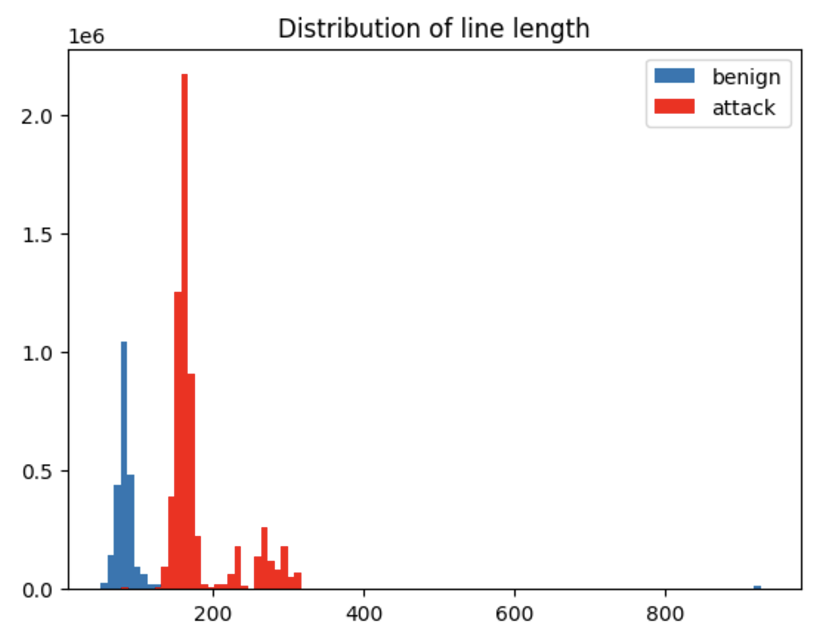
\includegraphics[width=0.8\textwidth]{linelength_distribution.png}
    \caption{Distribution of Log Line Lengths by Classification}
    \label{fig:linelength}
\end{figure}

\subsection{Model Development}

\subsubsection{BERT Tokenizer Customization}

We utilized HuggingFace's implementation of DistilBERT \cite{distilbert} and customized the tokenizer to handle system log syntax. Recognizing that logs differ from natural language, we fine-tuned the tokenizer on our dataset to better capture meaningful patterns.

\subsubsection{Model Training}

The training process involved:

\begin{itemize}
    \item Splitting the data into training, validation, and test sets.
    \item Employing oversampling and undersampling techniques to balance the dataset.
    \item Fine-tuning the BERT model using the customized tokenizer.
    \item Evaluating model performance using metrics such as accuracy, precision, recall, and F1-score.
\end{itemize}

\subsubsection{Baseline Models}

To establish a performance baseline, we trained simpler models, including logistic regression, random forest, and XGBoost classifiers, using engineered features like log line length and keyword presence.

\section{Results}

\subsection{Model Performance}

Our fine-tuned BERT model achieved the following results:

\begin{itemize}
    \item \textbf{Accuracy}: 99.7\%
    \item \textbf{Precision}: 99.6\%
    \item \textbf{Recall}: 99.5\%
    \item \textbf{F1-Score}: 99.6\%
\end{itemize}

These results significantly outperformed the baseline models, which achieved approximately 85\% accuracy on average.

\subsection{Analysis}

The high performance of the BERT model indicates its effectiveness in understanding and classifying complex log data. The model was able to learn intricate patterns and correlations within the logs that simpler models could not capture.

\subsection{Challenges and Solutions}

\begin{itemize}
    \item \textbf{Data Imbalance}: Addressed through resampling techniques.
    \item \textbf{Tokenization of Log Data}: Solved by customizing the tokenizer and fine-tuning on our dataset.
    \item \textbf{Pseudolanguage Complexity}: Overcome by training BERT to recognize the syntax and semantics of log data.
\end{itemize}

\section{Implementation}

\subsection{Full-Stack Framework}

We developed a robust architecture comprising:

\begin{itemize}
    \item \textbf{Backend}: Flask server managing API endpoints.
    \item \textbf{Database}: Redis for storing interim data and facilitating communication between components.
    \item \textbf{Frontend}: React-based interface for user interaction.
    \item \textbf{Model Integration}: Seamless connection between the frontend, backend, and the trained BERT model.
\end{itemize}

\subsection{Deployment}

The system was containerized using Docker and deployed on cloud platforms (e.g., AWS, Google Cloud) to ensure scalability and availability.

\section{Discussion}

\subsection{Impact and Benefits}

Our LLM-based NIDS offers:

\begin{itemize}
    \item \textbf{Enhanced Security}: Proactive detection of a wider range of threats.
    \item \textbf{Improved Efficiency}: Reduced false positives, lowering operational costs.
    \item \textbf{Future-Proofing}: Adaptability to new and evolving attack vectors.
\end{itemize}

\subsection{Cost Analysis}

An initial investment of \$10,000 was made for GPU resources. Compared to ongoing costs of leading NIDS contractors (up to \$576 per day), our system provides a cost-effective alternative, recouping the initial investment in a relatively short time frame.

\subsection{Limitations and Future Work}

While our system shows promising results, challenges remain:

\begin{itemize}
    \item \textbf{Continuous Learning}: Implementing mechanisms for ongoing model updates with new data.
    \item \textbf{Real-Time Processing}: Optimizing for low-latency detection in high-throughput environments.
    \item \textbf{Explainability}: Enhancing the model's ability to provide interpretable explanations for its detections.
\end{itemize}

\section{Conclusion}

We have developed a full-stack LLM network intrusion detection system that leverages advanced NLP techniques to analyze system and network logs as natural language. Our fine-tuned BERT model achieved 99.7\% accuracy in classifying network intrusions into six major categories. The system offers significant improvements over traditional NIDS in terms of accuracy, adaptability, and cost-effectiveness.

This project demonstrates the potential of LLMs in cybersecurity applications and sets the groundwork for further advancements in intelligent threat detection systems.

\section*{Acknowledgments}

We thank Sandia National Laboratories, particularly Ryan Holt and Mike Reed, for their support and collaboration. We also acknowledge the contributions of the INSyT team members: Bronze Frazer, Isaac Peterson, and Damon Tingey.

\begin{thebibliography}{9}

\bibitem{databreachreport}
IBM Security and Ponemon Institute. (2023).
\newblock \emph{Cost of a Data Breach Report 2023}.
\newblock Retrieved from \url{https://www.ibm.com/security/data-breach}

\bibitem{traditionalnids}
Garcia-Teodoro, P., Diaz-Verdejo, J., Macia-Fernandez, G., \& Vazquez, E. (2009).
\newblock Anomaly-based network intrusion detection: Techniques, systems and challenges.
\newblock \emph{Computers \& Security}, 28(1-2), 18-28.

\bibitem{anomalyissues}
Sommer, R., \& Paxson, V. (2010).
\newblock Outside the closed world: On using machine learning for network intrusion detection.
\newblock In \emph{2010 IEEE Symposium on Security and Privacy} (pp. 305-316).

\bibitem{neuralnids}
Kim, G., Lee, S., \& Kim, S. (2014).
\newblock A novel hybrid intrusion detection method integrating anomaly detection with misuse detection.
\newblock \emph{Expert Systems with Applications}, 41(4), 1690-1700.

\bibitem{bert}
Devlin, J., Chang, M. W., Lee, K., \& Toutanova, K. (2019).
\newblock BERT: Pre-training of Deep Bidirectional Transformers for Language Understanding.
\newblock In \emph{Proceedings of NAACL-HLT 2019} (pp. 4171–4186).

\bibitem{distilbert}
Sanh, V., Debut, L., Chaumond, J., \& Wolf, T. (2019).
\newblock DistilBERT, a distilled version of BERT: smaller, faster, cheaper and lighter.
\newblock \emph{arXiv preprint arXiv:1910.01108}.

\end{thebibliography}

\end{document}